\documentclass[header.tex]{subfiles}
\begin{document}
\title{\plaintitle}

\numberofauthors{3}
\author{%
  \alignauthor{Leave Authors Anonymous\\
    \affaddr{for Submission}\\
    \affaddr{City, Country}\\
    \email{e-mail address}}\\
  \alignauthor{Leave Authors Anonymous\\
    \affaddr{for Submission}\\
    \affaddr{City, Country}\\
    \email{e-mail address}}\\
  \alignauthor{Leave Authors Anonymous\\
    \affaddr{for Submission}\\
    \affaddr{City, Country}\\
    \email{e-mail address}}\\
}




\teaser{
%\begin{figure}
\centering

\includegraphics[width=0.9\textwidth]{figures/Fig1}
\caption{Sketch\&Stitch walkthrough: (a) A user sketches an art pattern directly on fabric, (b) shes uses \textit{Circuit Stickers} to plan and sketch the circuit, (c) she takes a picture of the design on fabric, (d) the system converts the design into embroidery patterns, and  embroidery machine stitches the patterns using conductive and non-conductive threads, (e) the user attaches electrical components in place of Circuit Stickers.
}
 \vspace{-1em}
\label{fig:Fig1}
}

\maketitle



\begin{abstract}
E-Textiles are fabrics that integrate electronic circuits and components. Makers use them to create interactive clothing, furniture, and toys. However, this requires significant manual labor and skills, and using technology-centric design tools. We introduce \textit{Sketch\&Stitch}, an interactive embroidery system to create e-textiles using a more traditional crafting approach: sketching on fabric. Users draw their art and circuit on fabric using colored markers. The system takes a picture of the sketch, converts it into embroidery patterns, and sends them to an embroidery machine. Alternating between sketching and stitching, users build and test their design incrementally. Sketch\&Stitch features \textit{Circuit Stickers} representing circuit boards, components, wire crossings to insulate, and various textile touch sensors such as pushbuttons, sliders, and 2D touchpads. Circuit Stickers serve as placeholders during design. Using computer vision, they are replaced later in the appropriate embroidery phases. We close with application examples.
\end{abstract}


\category{H.5.2}{User Interfaces}{}

\keywords{\plainkeywords}

\section{Introduction}


Electronic textile technology enables people to create expressive, interactive, and functional textile artifacts for both playful and serious applications.
It combines the visual and haptic expressiveness of textiles with the interactivity and utility of electrical components, e.g., LEDs, GPS sensors, vibration motors, speakers, touch sensors. At the intersections of technology, art, and fashion, e-textiles have attracted artists, designers, hobbyists, and makers to apply this technology in creative and artistic ways \cite{Buechley:2010:LWH:1858171.1858206,CuteCircuit}. 
%https://iq.intel.com/fashion-metamorphosis-meet-the-butterfly-dress/
%http://ezratuba.com/wearable-tech
This has motivated HCI researchers to investigate techniques that enable a wide audience to combine fabrics and electronics into interactive textiles \cite{Buechley2009,5387040}. 


In e-textiles, flexible conductive threads, inks, polymers, or  textiles are attached directly to the fabric. They are laid out to form \textit{fabric circuits}, electrical connections that transmit data and power between electrical components. 
They can also be manipulated to create fabric sensors [], resistors [], antennas [], batteries [], and other electronic units. The techniques for fabricating fabric circuits are based on traditional textile methods, such as weaving, knitting, stitching, and printing \cite{castano2014smart}. A typical walkthrough for creating e-textiles involves a) designing or choosing an art pattern, b) planning the circuit layout and placing the components, c) executing the pattern and circuit using the one of the above techniques, d) insulating the circuit, and e) attaching the electrical components \cite{Buechley2009}.



%Some of these techniques have been successfully adopted by the do-it-yourself community 
% as evident from makers' websites, such as Instructables\footnote{https://www.instructables.com/}, Sparkfun\footnote{https://www.sparkfun.com/} and Adafruit\footnote{https://www.adafruit.com/}. But these techniques have some constraints.
%More websites: https://www.lib.ncsu.edu/softcircuits



Current e-textile fabrication techniques are predominantly manual. As a result, executing a design can be labor-intensive and require high levels of skills, especially as the number and density of electrical connections and components increases. Debugging a fabric circuit is only possible after the user has invested considerable time in fabrication. In addition, current techniques demand a separate step, tools and materials for insulating the electrical connections, which is necessary for achieving a functional artifact. %preventing accidental contacts during fabric movement. 
Observing participants in our e-textile workshops, we found that this laborious multi-step process often forces people to make a trade-off between the visual and functional aspects of their design, and impedes improvisational fabrication. %people during early design explorations. 
%enable users to focus and invest their time on the visual and functional aspects of their project.


% We analysed more than 70 e-textile projects on the mentioned websites and found that makers make a trade-off between the fidelity of the artistic pattern and the functionality of the artefact. 


In this paper we propose utilizing a computerized embroidery machine as a digital fabrication tool for handling the laborious steps in e-textile creation---stitching and insulation. We introduce Sketch\&Stitch, an interactive embroidery system that enables users to create e-textiles by sketching on fabric (Fig.~\ref{fig:Fig1}). Th system features \textit{Circuit Stickers}, printed adhesives that represent elements that users can embed in their design, such as circuit boards, components, wire crossings to insulate, and various textile touch sensors. These stickers guide users while drawing circuit traces to ensure reliable electrical connections.

In Sketch\&Stitch, a user begins by sketching an art pattern on the workpiece fabric using colored fabric markers. She plans the placement of components using Circuit Stickers and draws connections. When the user is ready to execute the design, she takes a picture of the sketch, and the system converts it into embroidery patterns, and sends them to an embroidery machine. 
%The embroidery machine's embedded display allows the user to verify the patterns and make minor adjustments before stitching is started. 
The user may repeat these steps, adding and erasing  sketch markings, and debugging the circuit's function.  After embroidery, Circuit Stickers guide the user to attach the electrical components on fabric using one of three techniques we describe.

This paper makes the following contributions: 1) Sketch\&Stitch, a proof-of-concept systems for designing and executing e-textiles while directly working on the physical workpiece,, 2) embroidery techniques and patterns for stitching conductive traces, sensors, circuit bridges and insulation.






%In the remainder of this paper we present related work, followed by conductive embroidery techniques, a description of our system and a full design walkthrough, example artifacts created using our system, and finally a discussion of the limitations and future work of of this paper.





% Machine embroidery has bloomed entering homes, makerspaces and design studios of crafters, hobbyists and DIY.

% \url{http://www.strategyr.com/MarketResearch/Sewing_Machines_Market_Trends.asp}

% \url{http://robyns.world/2015/06/13/infographic-sewing-machine-day/}



\section{Embroidery Machine In Personal Fabrication}
Computerized embroidery machines became available for homes and small business in the 1980s. Today, they are part of maker-psaces, schools, libraries, and other creative scenes \cite{}. 
%An embroidery machine retails at 500 - 15,000 USD.
Embroidery machines use a hooping system to hold the framed area of fabric taut under the needle and move it automatically on an X and Y axis to stitch embroidery patterns. A presser foot, a metallic attachment that surrounds the needle, holds the fabric flat during embroidery to prevent it from rising and falling with the needle. A control panel and embedded display enable users to start-stop the machine, control thread tension, change stitching speed, view embroidery patterns and make minor adjustments (e.g., re-positioning, scaling, rotating, sequencing). Embroidery machines can stitch up to 1000 stitch/min.

An embroidery machine reads a digitized embroidery pattern %from a memory card, or via wired or wireless connection to a computer.
and generates a tool path. The path dictates how an embroidery hoop moves under the needle. It includes stitches, color changes, and jump stitches when traveling between different stitch objects. 
%While traveling, the needle is pulled up, and the presser foot hovers over fabric at a distance of about 1 mm.
A large number of jump stitches is a sign of bad design digitizing. Expert embroidery designers re-program embroidery patterns manipulating the sequence of individual stitches manually in order to influence the tool path and reduce jumps.

Embroidery machines come with proprietary software to optimize the digitization of designs for the machine. For example, 
%This process includes digitizing the image, and recognizing its color scheme to match it to thread colors. 
design objects that share a common color are stored in a single layer to be embroidered sequentially. %The embroidery machine recognizes the layers and stitches them sequentially,
The machine pauses between each two layers for the user to exchange threads. Virtual hoops help the user position, orient and scale a design relative to physical hoops. 
%Some software tools allow the user to print a design inside a virtual hoop in life-scale to assist the user in aligning the physical hoop on the workpiece fabric.

Similar to advanced CAD tools, embroidery software require a relatively steep learning curve. They offer a large number visual design options as well as specialized tools for manipulating stitch patterns, such as a parametric stitch designer. % and pull compensation options. 
In addition, the user-interface language of these tools is targeted at users who posses a level of knowledge in threads, fabrics, and embroidery.
%and the basic dynamics of the embroidery machine.


\subsection{Embroidering with conductive thread}

In this paper we use Bernina 880B\footnote{https://www.bernina.com/880} embroidery machine and software (DesignerPlus version 8) with Shieledx 117/17 dtex 2 ply silver sewing thread (linear resistance < 30 $\Omega$/cm). 
%http://www.shieldextrading.net/products/yarns-threads/
This thread can carry current for power and signals. The embroidery machine requires two types of thread: a top thread (or fashion thread) which appears on the surface of fabric, and a bobbin thread which runs on the wrong side of the fabric to pull the top thread down. We investigate using conductive thread as a top thread. While working with the conductive thread we adjusted the embroidery machine as follows: we set the stitching speed to 400 stitch/min to reduce the heat and friction that is associated with high speeds. We reduced top thread tension by 0.25 degrees from fabric recommendation. We used metallic thread needles and a light weight bobbin thread (60wt).


We conducted a battery of experiments to identify stitching parameters for conductive thread. 

\paragraph{Resisitivity}
\paragraph{Spacing}
\paragraph{Insulation}


% one of the few conductive threads commercially available for the sewing/embroidery machine. Other threads are \nur{TODO} The reason is  \nur{TODO}. In addition, threads must withstand the heat and friction that is associated with the high speeds of the embroidery process. More thread options (e.g., \nur{TODO}) are available for the bobbin. We found a speed of 700 stitch/min to work well with this thread. 




%What thread we used. What we learnt about tension, speed, metallic needles, stitch distance, decrease resistance.




\section{Sketch\&Stitch}
Sketch\&Stitch utilizes an embroidery machine to take over the laborious tasks in e-textile fabrication---stitching and insulating conductive traces. Yet, it maintains the physical and direct interaction between the user and the workpiece (fabric) during the creative tasks---designing and planning visual and functional patterns. 
%By this, the system aims to ... 
%reduce the entry barrier to e-textile fabrication and 
%encourage creative and improvisational and creative designs.

Sketch\&Stitch design pipeline was developed with designers and makers in mind. It enables them to convert a idea sketched on fabric into an interactive embroidery without having to interact with computer screens or CAD tools. Unlike circuit layout tools (e.g., Eagle or Fritzning), Sketch\&Stitch enables users to draw electrical connections in free artistic shapes adding a design interest to the circuit layout. Users interact with the system using colored markers and \textit{Circuit Stickers}. It is thus designed for improvisational and iterative prototyping during early design stages. 


%asses the visual design, test circuit layouts, or evaluate how the fabric material will behave when electrical components are attached to it
%It automizes the digitization of designs into embroidery patterns, and includes new patterns for conductive thread. 


Circuit Stickers are symbolic images printed on adhesive sheets of paper. They have the same shape, size and name of components they represent. Sketch\&Stitch defines two types of stickers: black stickers, which represent hardware electronics, such as circuit boards, LEDs, motors, speakers; and red stickers representing custom embroidery patterns for fabric circuit, e.g., touch sensors, and circuit bridges. Circuit Stickers are designed to help users plan and sketch a circuit with ease and precision. The adhesive backing invites for exploring different placement layouts, and holds the stickers in place during sketching and stitching. After embroidery, black stickers guide the placement (position and orientation) of their physical counterparts.
%Some stickers include grooves to guide users' traces to ensure reliable electrical connection with the added units. 


The general workflow of Sketch\&Stitch allows users to a) sketch art pattern directly on fabric with a textile marker, b) plan the placement of circuit elements using Circuit Stickers, and draw the connections between them, c) capture design on fabric with a camera, d) stitch the digitized patterns on the embroidery machine, and finally e) attach electronics onto fabric.

%  We aim to make e-textile creation accessible for emerging designers, hobbyists, crafters, and makers.
%To keep the traditional craft ways of entirely working on the physical workpiece, we developed a pipeline that enables users to sketch the design and plan the circuit directly on fabric. This pipeline 
% Simulating the traditional craft ways of directly interacting with the physical form using tools opens up a range of new creative possibilities [].
% Continuous representation of the object of interest.
% Allows designers/artists to establish a closer relation with materials to better understand their properties and nuances. Disconnect between physical and digital: There are numerous sources of variability in textile materials that can make a digital representation unstable, regardless of how good the simulation is.
% More agency and control over the final outcome [Being the Machine: Reconfiguring Agency and Control in Hybrid Fabrication].




\subsection{Sketching the design}
Drawing on fabric is an established form of art. It is also used to design patterns for manual embroidery. 
%Freehand sketching is the way users convey their design ideas to the system, and color, is the interaction language. 
Sketching on fabric, like sketching on paper, utilizes a simple and masterful tool, a marker, to enable users to express themselves freely without the constraints of design applications \cite{schweikardt2000digital}. Physical sketching provides users with direct feedback on how a design (i.e., position, orientation, scale) will appear on the workpiece fabric. 
Before sketching, a user secures the workpiece fabric in an embroidery hoop of a desired size. The hoop hold the fabric taut during sketching and frames the design location on the workpiece. 
Using washable fabric markers, users draw and modify their sketches. One marker color is dedicated for art pattern to be stitched with non-conductive thread. A second color is used to draw circuit traces and sensors to be stitched with conductive thread. %The user can draw any lines and shapes. 
The user can start with either the art or circuit pattern, and alternate between them. If the users wants to \textit{undo} any of the markings, she can simply pat on them with a damp piece of cloth. 
 
 \begin{figure}
\centering
  \includegraphics[width=0.7\columnwidth]{figures/Spacing}
  \caption{}~\label{fig:Spacing}
  \vspace{-2.5em}
\end{figure}

While sketching circuit traces, the users should maintain a minimum of 2.5 mm spacing between adjacent conductive traces. Figure \ref{fig:Spacing} depicts our experimentation with different spacings (1, 1.5, 2, 2.2, 3, and 3.5 mm). Traces spaced at 2 mm were not electrically connected when we first started the experiments. But as we handled the fabric repeatedly, the conductive thread started to fray, and 2 mm spacing was not enough to prevent adjunct lines for coming in contact. 

User design does not need to be complete before it can be stitched. At any point in design, the user can take a picture of the fabric, secure the hoop in embroidery machine, and start the stitching process. This enables users to evaluate and test their design early on. Users can then proceed, \textit{incrementally} sketching and designing on fabric.
%To support incremental design, users must avoid using threads fom the system's color scheme.


\subsection{Insulating circuit traces}
\begin{figure}
\centering
  \includegraphics[width=0.7\columnwidth]{figures/Insulation}
  \caption{}~\label{fig:Insulation}
  \vspace{-2.5em}
\end{figure}
Insulating circuit traces, especially in wearable e-textiles, is paramount for their functionality. Textiles are flexible materials. Exposed traces may come in contact with each other as fabric folds or bends creating shorts or undesired signals.


%Buechley et al. [] described three materials that can be used to insulate conductive fabric traces: puffy fabric paint, non-conductive iron-on fabric, and non-conductive thread. 

Buechley et al. [] proposed couching---stitching one thread over another---as an organic insulation technique for fabric circuits. However, they noted that sewing machines may leave gaps in the top stitch making it an unreliable cover for the underlying conductive thread.

Computer-controlled embroidery machines are particularly more qualified than sewing machines at maintaining a consistent couching stitch. The zigzag stitch is the most commonly used stitch for couching. It is defined by two main parameters: width of the stitch and spacing between threads (density). We manipulated these parameters to find the stitch that best insulates a triple running stitch of conductive thread. Insulating conductive thread is challenging due to its fraying properties. Our goal was to find a trade-off between the reliability of insulation, and the width and destiny of the stitch. A wide insulation stitch would dictate the smallest distance between adjunct traces and might have a pounced visual effect on the design. A highly dense stitch requires more thread and could reduce the flexibility of the underlying fabric, especially if applied to several traces in a small area.

We evaluated the reliability of insulation stitches as follows: we overlaid the insulated traces over non-insulated conducive traces, and applied different amounts of pressure (0.2, 0.6, 2, 6, 10, 14, 18 N) at 5 equidistant points along each trace. Figure \ref{fig:Insulation} summarizes the results. We found that a zigzag stitch of 2.0 mm width and 0.4 mm spacing satisfies our technical and design requirements. Based on this results, two insulated traces can be spaced 2 mm apart.

In Sketch\&Stitch, a user can selectively insulate circuit traces by drawing them with a distinct marker color, e.g., green.

%The system creates two duplicate files for all markings in C: one file tints the markings with grey, and the other file tints the markings with yellow. As mentioned previously, the colors are matched to predefined stitches, in this case triple run and zigzag (x,y), respectively, and are sequenced for execution in a predetermine order.


\subsection{Handling Crossing Traces}
\begin{figure}
\centering
  \includegraphics[width=0.7\columnwidth]{figures/BridgeStitch}
  \caption{}~\label{fig:BridgeStitch}
  \vspace{-2.5em}
\end{figure}
As the number of circuit elements increases in a design, traces crossing each other become inevitable. 

%Dunne et al. [] manipulated the tension of thread to allow two conductive threads to crisscross without coming in contact with each other. However, this technique does not provide a fail-safe insulation---when pressure is applied over the intersection point, traces can come in contact with each other. In addition, various fabric-thread combinations require different tension settings and changing these settings may affect the appearance and strength of the stitches. 
Building on the insulation stitch describe above, we developed the \textit{bridge stitch}, an M shape stitched with a single running stitch (length: 9 mm) and tie-on and -off thread securing knots on different ends. It is used to connect the two separate traces (< 9 mm apart) without stitching between.

Figure \ref{fig:BridgeStitch} illustrates a bridge pattern. The pattern is composed of three embroidery layers: bottom layer is a conductive line connecting the ends of a cropped trace, the middle layer is a 3.7 mm long insulation stitch, and the top layer is a bridge stitch.

We designed a bridge circuit sticker that the user can adhere over crisscrossing traces to signify a bridge pattern. The sticker has groves to guide user traces. This ensures that the bridge patterns with overlap with the traces. Self crisscrosses of conductive thread are safe and do not need to be handled.

%When the system filters for the color of this sticker, it replaces it with three design layers: layer of the condutive traces (Figx1), layer for the insulation (Figx2), and layer for the conductive bridge (Figx3). The conductive brideg is designed to be 1.5 times longer than the physcal gap in order to create some overlapping witches with the ends of the disconnected trace. It is repaeted 5 times to create a song connection. \nur{using a jump also works but is can be loose, snatch and cut}. Figx3 is tinted with darker grey. Markings tinted with dark gray are sequnaced last in the embroidery queue.


\subsection{Adding Electronics}
Embroidering while hardware components are on fabric is very challenging for most embroidery machines due to the presser foot hovering range (~ 1 mm). For context, LilyPad PCBs are 0.8 mm thick, but with attached SMD components the total thickness is more than 2 mm. Additionally, when working with hardware on fabric, a 1 mm miss-alignment between the virtual and physical sketch can lead to needle or electronics breakage. 

To overcome this hurdle, we designed a set of Circuit Stickers to represent the physical components that users can add to their design. Figure \ref{fig:BlackStickers} shows the stickers for some of the LilyPad components. Circuit Stickers can be created for any component with contact pitch of 2.5 mm. 
\begin{figure} [h!]
\centering
  \includegraphics[width=0.5\columnwidth]{figures/BlackStickers}
  \caption{}~\label{fig:BlackStickers}
  \vspace{-2.5em}
\end{figure}


\subsection{Adding Interactivity}
\begin{figure}
\centering
  \includegraphics[width=0.6\columnwidth]{figures/RedStickers}
  \caption{}~\label{fig:RedStickers}
  \vspace{-2.5em}
\end{figure}
Besides hardware electronics, the embroidery machine can stitch simple electrical components using only conductive thread. Below we three embroidered touch sensors: a push button, a 1D slider, and a 2D touchpad (Figure \ref{fig:RedStickers} .
%actuators, e.g., by couching a shape memory alloy wire, and various touch sensors, as we will demonstrate in this section.

The pushbutton, is the simplest sensor---by connecting a piece of conductive thread to a capacitive sensing circuit, a pushbutton is created. The circuit can sense when the user's finger or body is in contact with the thread (touch) or not (no touch). A resistive pushbutton can be created by stitching two conductive threads near each other and connecting one thread to ground and the other one to power. When the user touches the two line at the same time, a resistive sensing circuit registers a touch.

A 1D slider can be implemented using several pushbuttons places next to each other. By connecting these buttons to a capacitive circuit, we can expand beyond push buttons with on/off functionality, to interpolate the position of the contact based on the amount of surface area the contact covers as well as its influence on the capacitance of neighbouring buttons.

% to determine more than one capacitive threshold for a single button. As the user's body comes in contact with more surface o with a capacitive sensor is interacted with by the user, the larger the capacitance will be. 

A matrix of buttons, where each button is connected to one pin, offers the ability to detect all buttons being pressed at the same time, i.e., multi-touch. However, a 4 by 4 touchpad will require 16 IO pins and traces. This can complicate the wiring and require additional hardware. Instead, using a grid layout provides a sensor surface area that is capable of detecting individual buttons, simple gesture analysis, and sub-sensor point detection that can be used for trackpads. A grid sensor requires fewer IO pins (8 in case of 4 by 4 pad) and lower power than the individual button scanning. However, it cannot support multi-touch. A grid layout can be connected to a capaciiuve or resistive circuits. But due to the low resistivity of the human finger, not all hardware can detect a direct touch. One alternative is to use pinching as an input technique. Hamdan et al. [] were able to detect the location and angle of a pinch on a matrix of resistive textile buttons using simple machine learning algorithms.


The user can create a single pushbutton by extending a piece of conductive fabric and manipulating it in any motif. Two traces 2-3 mm apart are needed for a resisitive button. For 1D sliders and 2D touchpads, we designed a red Circuit Sticker that can be printed on a sheet of adhesive paper, cut into any convex shape, adhered to fabric, and connected to a sensing board with skectched conductive traces. The sticker includes faducial markers that represent a bridge pattern. Once the system captures the sticker on fabric, the user removes, and the machines embroiders it in place.
%The grid was designed based on the recommendation of Texas Instruments []




% constructed by “opening up” a capacitor structure so that the
% electric field can be interfered with by a conductive foreign object, in this case, a fingerWhen a conductor, e.g., a finger,
% comes into the area above the open capacitor, the electric field is interfered with causing the
% resulting capacitance to change. The coupling of the conductive finger into the capacitive sensor
% increases the capacitance of the structure beyond the baseline capacitance, the capacitance of
% the sensor with no touch. By continuously measuring the capacitance of the sensor(s) in the
% system and comparing each result to a predetermined baseline capacitance, the system
% microcontroller can determine not only on/off button functions for each sensor element but also
% “amount” of press used for more complex interfaces such as positional sliders. 
% The base capacitance of such a design is affected by stray capacitances on the PCB as well as
% potentially other environmental effects such as temperature and humidity. Therefore, the
% detection system needs to constantly monitor and track this variation for correct comparison to
% touch events. 



\subsection{Attaching Electronics}
%We mainly considered sewable components, and components with flat pads on the wrong side of the unit.




After embroidery, the user replaces Circuit Stickers with hardware electronics. The design pipeline simplifies this step by preparing the contact points. 
%Attaching hardware circuit boards and components to fabric is one of the main challenges in e-textiles. Researches have explored several techniques including soldering [], special soldering [], manual sewing [], breads [], ...
For Sketch\&Stitch user, we describe three techniques: First technique uses M3's Z-tape, a double sided adhesive that conducts in the Z-dimension when pressure is applied. Z-tape is applied to the wrong side of a component. The components is adhered and aligned over the stitched contact points. By pressing the component on fabric, connections between pins and connective contacts are created. This technique is suitable for prototyping and testing the circuit as well as for fabrics with low movement requirements. 

%We do not know if Z-tape can hold components with legs, we only tested with flat pads.

\begin{figure}
\centering
  \includegraphics[width=0.7\columnwidth]{figures/LilyStitch}
  \caption{}~\label{fig:LilyStitch}
  \vspace{-2.5em}
\end{figure}

The second technique utilizes an embroidery machine. We developed the \textit{Lily stitch} (Fig. \ref{fig:LilyStitch}. A stitch tailored for attaching LilyPad components of 3 mm diameter hols. The stitch is an M shape (height: 9 mm, width: 0.8-1.2 mm) stitched with a single running stitch (length: 9 mm), and tie-in and -off knots on one end. 
%Tie knots need space that 3mm is not encough for them
The height of the lily stitch accounts for a) distance between the center of a pin hole and outer edge of the PCB (\~ 4 mm), and b) distance between needle point and presser foot outer edge (\~5 mm). 
%Reducing the stitch distance will lead the presser foot to push against the edge of the PCB when stitching close to it. On the other hand, increasing the distance can weaken the strength of the connection.

Fig X, shows a custom embroidery pattern for embroidering Arduino USB - ATmega32U4 Board. The sequence of stitches was modified manually to prevent the presser foot from traveling over the component during embroidery. This technique is very reliable and efficient for attaching sewable electronics. However, it requires a millimeter accurate alignment between the physical component on fabric and the embroidery pattern. If an embroidery machine does not support such accuracy, one can start by stitching part of this pattern on fabric, align the component on fabric based on the stitches, and restart the pattern embroidery.
%We recommend embroidering the hardware after the art and circuit patterns have been fully embroidered to avoid travel stitches.

The last technique is using the button sewing foot in sewing machines and manually align the holes of sewable components under the foot. This technique requires some skill than manual sewing but it can be more efficient. 
%And part stickers
The results of sewing machine and manual sewing can be as  reliable as the embroidery machine's but require more labor and time compared to the other techniques.  

\subsection{Concealing Traces and Components}
Our system offers three techniques to conceal fabric circuits and hardware components in a design: the first is drawing circuit traces close to art outlines. 
%The spacing constraint of 2.5 mm need not to be applied between conductive and non-conductive threads. 
While this technique might not hide the traces completely, it will make them less visible and obvious since the width of art stitches is relatively larger.

The second technique is camouflaging traces by insulating them with a thread color that matches the color of fabric []. Traces will not be hidden completely, but depending on the desired application, this technique may be sufficient to occlude electrical connections. 

The third technique allows users to hide fabric circuits and hardware components completely. This technique uses two pieces of fabric: one for sketching art pattern (top fabric), and one for sketching fabric circuit and adding part stickers (bottom fabric). The two fabrics are captured and embroidered individually. At the end of embroidery, hardware electronics are attached to the bottom fabric, and the top fabric is layered over it manually. This technique can also be used to create multi-layer textile circuits [], with an additional if an insulator, e.g., non-conductive fabric, between any two conductive layers. 







\section{Walkthrough: Fabric Drums}

\begin{figure}
\centering
  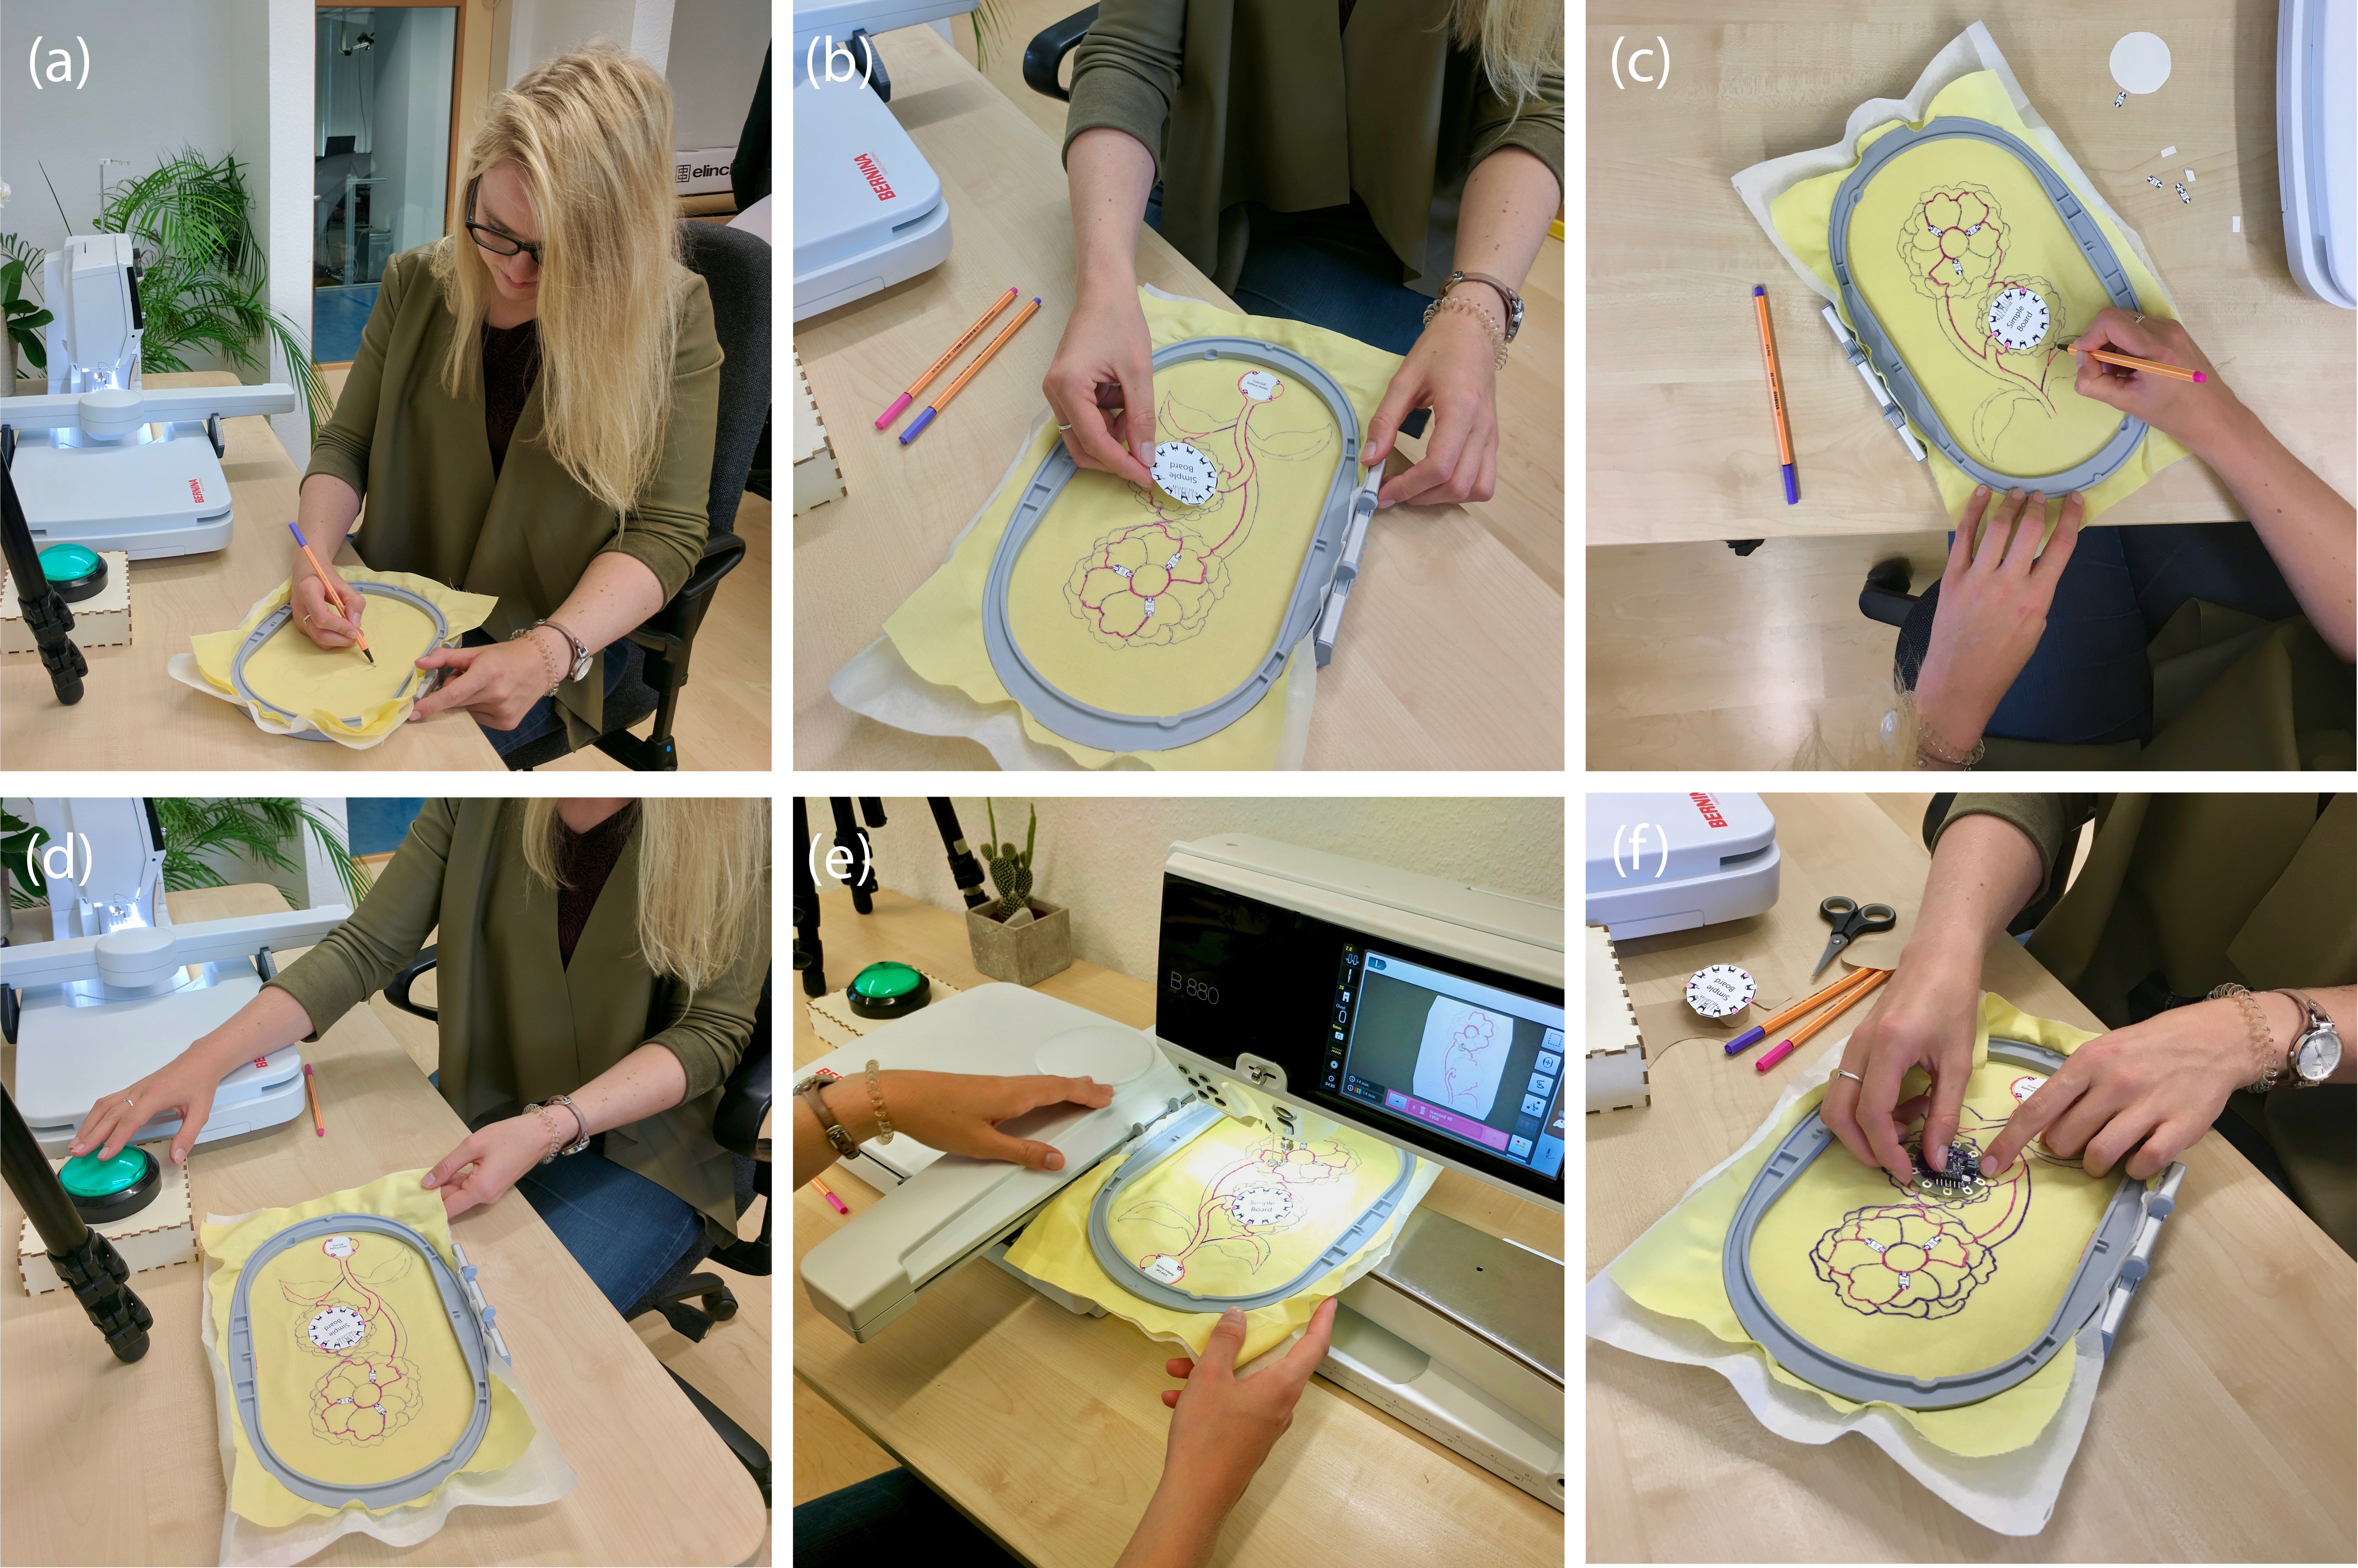
\includegraphics[width=0.9\columnwidth]{figures/Walkthrough}
  \caption{}~\label{fig:Walkthrough}
  \vspace{-2.5em}
\end{figure}
In the following, we illustrate Interactive Embroidery pipeline at the example of a fabric drums poster (inspired by Kate Stone's work in TED2013). The poster has 7 touch-enabled drums, a volume controller with 5 feedback LEDs, and an on/off switch button. Figure X shows the final outcome and the intermediate steps required to produce it.


\subsubsection{Materials and Preparation}
To fabricate the e-textile, the user needs the following materials: the workpiece fabric, two washable fabric markers of distinguishable colors, the electrical components, the component placeholders, and Z-tap (optional). For this poster project the following LilyPad Arduino electrical components are used: a controller ( x pins), speaker, 5 LEDs (3 white and 2 red), a switch button, and a battery. The users secures the fabric in an embroidery hoop in preparation to start the design.

%\nur{We are no including ``making the placeholders'' as part of the walkthrough.}

\subsubsection{Sketch}
The user begins by directly drawing on the workpiece fabric using a washable fabric marker. She picks up a purple marker and starts drawing the visual design pattern of the poster (Figure X). The user then places the electronics on the fabric to plan the fabric circuit (Figure X). Once she is satisfied, she replaces the electronics with their counterpart placeholders and sticks them on the fabric. To draw the touch-enabled drums and connections between the components, she picks up a blue marker and draws on fabric where the conductive thread should be stitched (Figure X). The user extends the connections inside the guiding gaps of the placeholder. For touch-enable areas, e.g., drums, the user draws multiple lines to increase the interaction surface of the sensor. If the user wishes to \textit{undo} any of her markings, she can simply rub the fabric with a small piece of damp cloth.

\subsubsection{Capture} 
When the user is ready to embroider her design, she takes the hooped fabric and places it under the capture system. A picture is take of her sketch. In a few seconds, she receives auditory feedback notifying her that her designs are transfered to the EM and ready to be stitched. She can then verify her designs via the built in display of the EM. %The display shows three files: sketch-purple, sketch-blue, and insulation-blue. She can verify whether all her markings have been captured and converted correctly. 
She can also use the EM built-in controls to manipulate the location, size, rotation, or create repeated patterns of her designs. If the user wishes to make changes to her design before stitching, she can simply draw/erase markings on the fabric and then capture the new drawing once more. The EM retains all captured designs enabling the user to choose the one that better satisfies her goals.

\subsubsection{Stitch}
To start embroidery, the user secures the embroidery hoop in the EM. She uses the machine's embedded display to verify her designs and chooses to stitch the circuit embroidery pattern first. This will allow her to debug the connections early on. She threads the needle with the conductive thread and starts the machine. Once the pattern is stitched, the machine stops. The user takes out the fabric to test the connections and trims any excess thread with scissors. The user decides to add another connection to her circuit. She places an additional LED placeholder on the fabric and uses the blue marker to draw the new connections between the LED and the controller. She then captures the design again. On the EM display she chooses the embroidery pattern that contains the recent markings and proceeds with embroidery. The user chooses not to insulate the circuit, and starts embroidering the artistic pattern.

\subsubsection{Attach Electronics}
Post-embroidery the user must trim excess threads, and test the circuit for shortcuts and undesired contacts. For rapid prototyping purposes, the user cuts a piece of Z-tape to match the shape and size of her electronics and attaches it to the bottom of the electronics. Guided by the placeholders, she determains where each component should go and replaces the placeholder with its physical counterpart.  Finally, the user can use software tools such as X and Y to program the functionality of her final circuit.



%The user is free to perform this step in any environment since her input is not tracked in real-time. 



\section{Example Projects}

\subsection{Nap Pillow}
Furniture.

Buzzer the starts if sensors detect contious contact for more than an hour. (Timer programmed via app.)

Hidden electronics.

\subsection{Interactive Desk Mat}
Leather fabric, large object, furniture.

Pomadoro interface of leds and switch button.
\subsection{Wearable Light}
Wearable, detailed art. (Video figure)

A sketched tree with LED leaves, flicker based on accelerometer.
\subsection{Pet the Cat}
Toy, stuffed cat, add interactivity to exiting objects. 

1D slider, reacts with sounds to the speed and direction of swipes.

Hidden electronics.



\subfile{Implementation}

\section{Design Benefits and Limitations}
% Our capture system cannot distinguish between overlapping lines in a single connection and between two connection. 

% The user has to make the 2 mm constrains her self. As we emphasize the artistic dimension of e-textiles and any system enforced changes can affect the integrity of the design.

% A single stitch type of the lines and the fillings.



% Some industrial embroidery machines, e.g., X, can stitch beads directly on the fabric. A container for beads attached near the presser-foot releases a bead on the fabric and stitches it based on a computer program---a pick and place machine for textile embellishment.

% \nur{Limitation and future work: we only focused on the top thread in this paper, next we will explore techniques for the bobbin as conductive thread.}}

\section{Conclusion and Future Work}
% BALANCE COLUMNS
\balance{}

% REFERENCES FORMAT
% References must be the same font size as other body text.
\bibliographystyle{SIGCHI-Reference-Format}
\bibliography{sample}

\end{document}
%%% Local Variables:
%%% mode: latex
%%% TeX-master: t
%%% End:
